\chapter{Implementation}\label{chap:impl}
The separation kernel design specified in chapter \ref{chap:design} has been
implemented in a functional prototype. This chapter presents the implementation
by first describing the system policy. The Ada Zero Footprint Runtime required
to compile the Muen kernel and subjects implemented in SPARK/Ada is outlined in
section \ref{sec:zfp-rts}. The following section \ref{sec:impl-subject}
introduces the data types used to manage subject specifications and subject
state in the Muen kernel. The kernel implementation is then presented in
section \ref{sec:kernel}. In order to build the kernel and subjects, a build
system with the appropriate toolchain is required. The build system
implementation is examined in section \ref{sec:build}. The chapter concludes by
presenting the Muen example system, which demonstrates the usability of the
separation kernel implementation.

\section{Policy}
All aspects of a system using the Muen kernel must be specified in a policy XML
file. The policy is composed of the following main parts:

\begin{itemize}
	\item Hardware
	\item Kernel
	\item Binaries
	\item Subjects
	\item Scheduling
\end{itemize}

XML was chosen as a specification language since it is human-readable and can
be automatically verified against a schema. Furthermore, there is an existing
Ada library called XML/Ada TODO:Ref, which is opensource and freely available.

Since XML processing is not done by any trusted part of the system, the policy
contained in an XML file is transformed into SPARK source using the policy
compilation tool \texttt{skpolicy}. This process is described in detail in
section TODO:Ref.

Each of the main policy parts is presented in the following sections. Preceding
these descriptions is the specification of data types, which are the basis for
the subsequent definition of policy elements. The data types and elements map
directly to their corresponding XML schema definitions.

\subsection{Data types}
This section describes basic data types that are used in the specification of
the system policy. They are referenced in later chapters, illustrating different
parts of the policy.

\input{types.tex}

\subsection{Hardware}
\label{subsec:hardware}
\begin{figure}[h]
	\centering
	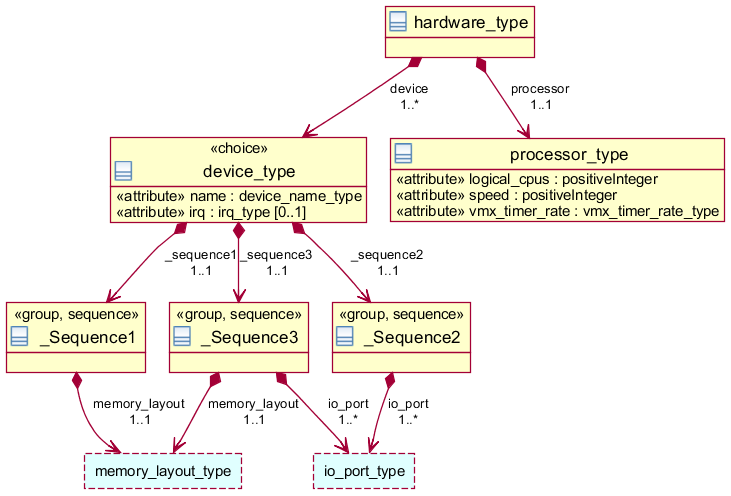
\includegraphics[width=\textwidth]{images/xml_hardware.png}
	\caption{Hardware policy}
\end{figure}
\input{hardware.tex}

\subsection{Kernel}
\begin{figure}[h]
	\centering
	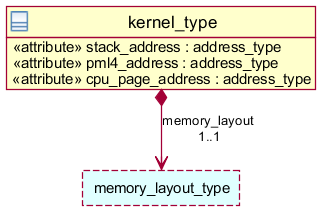
\includegraphics[scale=0.6]{images/xml_kernel.png}
	\caption{Kernel policy}
\end{figure}
\input{kernel.tex}

\subsection{Binaries}
\begin{figure}[h]
	\centering
	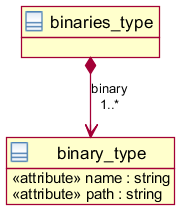
\includegraphics[scale=0.6]{images/xml_binary.png}
	\caption{Binaries policy}
\end{figure}
\input{binary.tex}

\subsection{Subjects}
\begin{sidewaysfigure}[hp]
	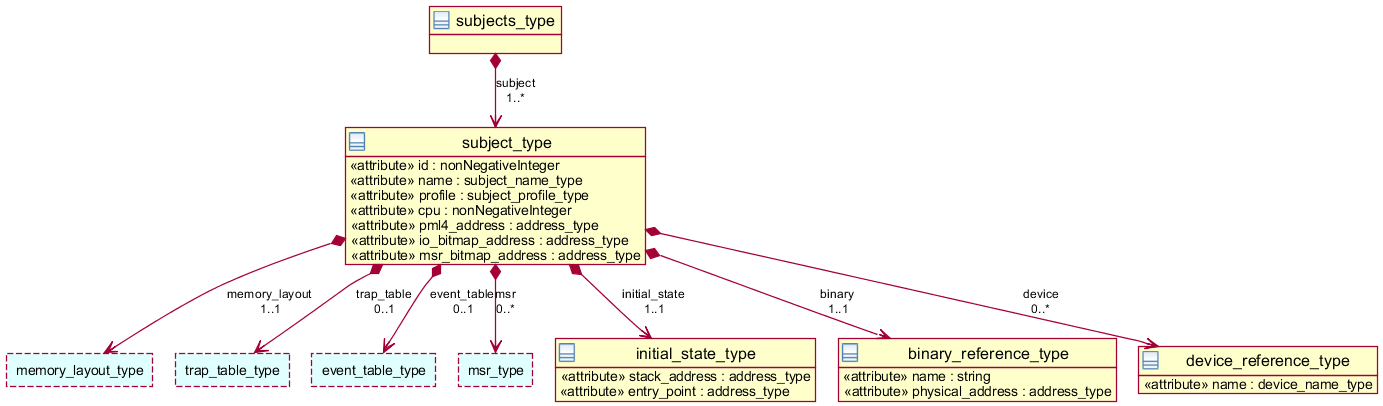
\includegraphics[width=\textwidth]{images/xml_subject.png}
	\caption{Subjects policy}
\end{sidewaysfigure}
\input{subject.tex}

\subsection{Scheduling}
\begin{figure}[h]
	\centering
	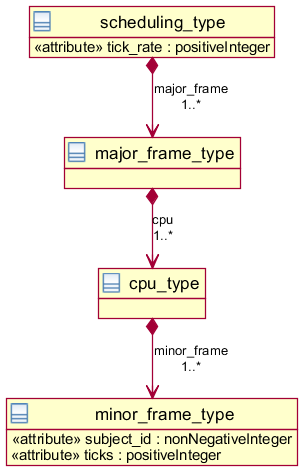
\includegraphics[scale=0.6]{images/xml_scheduling.png}
	\caption{Scheduling policy}
\end{figure}
\input{scheduling.tex}

\section{Zero Footprint Runtime}\label{sec:zfs-rts} To allow a minimal TCB for
the kernel and subjects, a special stripped-down version of an Ada
runtime\index{runtime} is provided by the Muen project. This runtime system
(RTS\index{RTS}) only contains the minimal Ada packages required to compile Ada
code for Muen. An Ada runtime system with such a minimal "footprint" is called
Zero Footprint Runtime (ZFP\index{ZFP}). The following is a list of currently
supported packages and functions:

\begin{itemize}
	\item function \texttt{Ada.Unchecked\_Conversion}
	\item package \texttt{Interfaces}
	\item package \texttt{System}
	\item package \texttt{System.Machine\_Code}
	\item package \texttt{System.Storage\_Elements}
\end{itemize}

These files have been extracted from the latest sources of the GNU Compiler
Collection (GCC\index{gcc}, \cite{gcc}) and are linked into a static library.
The runtime is then used to compile the Muen kernel and all subjects running on
the kernel.

Since the ZFP runtime has only a very limited set of Ada features available,
code using this runtime must be also very simple. Simple code is an important
pre-condition for formal verification of code.

The compliance of the Muen kernel to the SPARK\index{SPARK} language rules
already assures that no advanced Ada features are used. Additional restriction
pragmas\index{pragma} confine the language subset even further. The currently
used restrictions are shown in listing \ref{lst:pragmas}.

\lstinputlisting[
	language=Ada,
	label=lst:pragmas,
	caption=Restriction pragmas]
	{../config/restrictions.adc}

Details about restriction pragmas and their impact on the allowed Ada language
subset can be found in the GNAT Refernece Manual, section "Standard and
Implementation Defined Restrictions" \cite{GNAT:manual}.

\section{Subject}\label{sec:impl-subject}
Subjects are the main components that are executed on top of the kernel, as
described in section \ref{sec:design-subject}. They are represented using two
main data structures: subject specification and subject state.

\subsection{Specification}
A subject is specified in the global system policy. The XML specification
precisely defines the execution environment and granted resources. The
information that is relevant to the kernel is part of the compiled policy.
Listing \ref{lst:skp-subjects} presents the SPARK type specification into which
all subject specific policy parts are transformed. The specification of a
subject is static and cannot be changed at runtime.

\lstinputlisting[
	language=ada,
	linerange={14-33},
	label=lst:skp-subjects,
	caption=SPARK subject spec type]
	{../tools/policy/templates/skp-subjects.adb}

\subsection{State}
The system state related to a subject must encompass all resources that it can
control directly or indirectly. This is necessary to enable the scheduler to
preempt a subject by preserving its state and seamlessly resume execution at a
later stage by restoring the previously saved state.

Additionally, separation of subjects demands that unintended information flow
due to subject switching must be prevented. This is only achievable if the
subject state that is saved and restored encompasses every element of the
systems environment that is accessible by more than one subject. While the Intel
VMX extensions save and restore parts of the subject state automatically to and
from the associated VMCS on VMX transition, others must be handled manually by
the kernel. Listings \ref{lst:sk-subject-state} and \ref{lst:sk-cpu-registers}
show the record types used by the Kernel to maintain the state of a subject.

\lstinputlisting[
	language=ada,
	linerange={39-56},
	label=lst:sk-subject-state,
	caption=SPARK subject state type]
	{../common/src/sk.ads}

\lstinputlisting[
	language=ada,
	linerange={18-35},
	label=lst:sk-cpu-registers,
	caption=SPARK CPU registers type]
	{../common/src/sk.ads}

A SM\index{SM} subject may access the state of a given subject. This enables
the SM to alter a subject's state and thus perform emulation. Because a subject
is not allowed to access the VMCS structure of another subject, the kernel also
copies register values managed automatically by VMX\index{VMX} into the
in-memory subject state to enable modification by the SM subject.

During subject setup, the state is first set to a pristine value. This is done
by assigning the \texttt{Null} subject state constants shown by listings
\ref{lst:sk-null-subject-state} and \ref{lst:sk-null-cpu-registers} to all
state variables.

\lstinputlisting[
	language=ada,
	linerange={85-100},
	label=lst:sk-null-subject-state,
	caption=SPARK null subject state constant]
	{../common/src/sk.ads}

\lstinputlisting[
	language=ada,
	linerange={102-118},
	label=lst:sk-null-cpu-registers,
	caption=SPARK null CPU registers constant]
	{../common/src/sk.ads}

The initialization of the subject state is then completed by copying the code
entry point and the address of the stack from the specification.  These values
are declared in the system policy as part of the subject initial state and can
be obtained automatically from a native subject binary by using the
\texttt{skconfig} tool (see section \ref{subsec:subject-binary-analysis}).


\section{Kernel}\label{sec:kernel}
The following sections outline the implementation of the Muen separation
kernel.

\subsection{Init}\label{subsec:init}
After reset of a x86 system, the processor begins executing code at physical
address \texttt{ffff:0000}, which is mapped to the PC
BIOS\index{BIOS}\footnote{Basic Input/Output System}. The BIOS first performs
tests and initialization routines and then searches for a bootable storage
media. If found, the BIOS copies the first sector of the storage media to
physical address \texttt{0000:7C00} and jumps to this address (i.e. starts
executing code at this address). This is where the system bootloader comes to
live which is responsible to boot operating systems according to its
configuration. Many bootloaders first load additional code from the storage
media and then prepare the environment for OS execution.

The Muen seperation kernel is compliant to the multiboot specification, version
0.6.96 \cite{multiboot}. The multiboot standard is used to uniformly boot
different operating system kernels by multiboot-aware bootloaders.
The Muen kernel exports the required multiboot header within the first 8192
bytes of the OS image. The bootloader loads the OS image into memory according
to the information found in the header and jumps to the physical kernel entry
point specified in this header.

\begin{figure}[h]
	\centering
	\begin{bytefield}{24}
	\bitbox[]{10}{}
	\bitbox[]{16}{$\vdots$}\\[1ex]
	\memsection{0010 0000}{0020 3fff}{6}{Kernel memory}\\
	\memsection{0000 8000}{000f ffff}{3}{\color{Gray}-- free --}\\
	\begin{rightwordgroup}{VMX regions}
		\memsection{0000 5000}{0000 7fff}{2}{\color{Red}VMCS}\\
		\memsection{0000 1000}{0000 4fff}{2}{\color{Red}VMXON}
	\end{rightwordgroup}\\
	\memsection{0000 0000}{0000 0fff}{2}{\color{Red}AP trampoline}
\end{bytefield}

	\caption{Memory layout on system init (example)}
	\label{fig:init-mem-layout-example}
\end{figure}

Figure \ref{fig:init-mem-layout-example} shows the physical memory layout of an
example system. The kernel entry point of this system is at physical address
\texttt{0x00100000}. The main kernel uses the memory region starting from this
address to pysical address \texttt{0x00203fff} for code and data.

Low-memory (the physical memory below 1 MB) is used for system data structures
(colored in red). The AP\index{AP} trampoline\index{trampoline} is needed to
bootstrap the system's application processors as described in section
\ref{subsec:mp-support}. It initially resides in the kernel's text section and
must be copied to low-memory by the init code (see below).

To enable VMX operation using the \texttt{VMXON} instruction, one page per
logical CPU is required. This region is called VMXON\index{VMXON} region. Each
subject is managed using a VMCS\index{VMCS} data structure, so this memory is
placed in low-memory as well.

It is the bootloader's task to prepare the system state as demanded by the
multiboot standard, see \cite{multiboot} section 3.2 for details. The system
kernel can except the system to be in this exact state. After the Muen kernel
comes to live, it performs additional steps before jumping into the main SPARK
kernel.  This initial startup code is written in Assembly and conducts the
following tasks:
\begin{enumerate}
	\item Copy the AP trampoline to low-memory, see section
		\ref{subsec:mp-support} \item Initialize per-CPU VMXON regions
	\item Initialize subject VMCS regions
	\item Enable PAE\index{PAE}\footnote{Physical Address Extension}
	\item Initialize per-CPU kernel pagetables
	\item Enable IA-32e mode and execute-disable (NX)
	\item Enable paging, write protection, caching and native FPU error
		reporting
	\item Set up 64-bit GDT\index{GDT}\footnote{Global Descriptor Table}
	\item Set up Page-Attribute Table (PAT)
	\item Set up kernel stack
	\item Initialize Ada runtime
	\item Jump into kernel main
\end{enumerate}

The system is now in 64-bit IA-32e mode and each kernel calls the \texttt{VMXON}
VT-x instruction to enter VMX root operation.

\subsection{Multicore support}\label{subsec:mp-support}
The Muen separation kernel makes use of all logical processors available in a
system. The processor count of a specific hardware platform is declared in the
system policy, see section \ref{subsec:hardware}. This section describes how
the multicore setup is done during kernel startup.

Modern PC systems comply to the Intel MultiProcessor (MP\index{MP})
specification. In short, the Intel MP specification is an open-standard
describing enhancements to both operating systems and firmware to be able to
inititialize, boot and operate x86 multiprocessor systems. For more information
see \cite{intel:mp}.

After the hardware completed its part of the MP specification, one processor
has been negotiated to be the bootstrap processor (BSP\index{BSP}). All other
logical processors, called application processors (AP\index{AP}), halt until
they receive a specific inter-processor interrupt (IPI\index{IPI}) sequence.

\begin{figure}[h]
	\centering
	\begin{tikzpicture}
	\node[greenbox, minimum width=9cm] (mem) {System Memory};

	% SK 0
	\node[graybox, minimum width=2.8cm, below=1cm of mem.south west, anchor=north west] (pc1) {Per-CPU storage};
	\node[graybox, minimum width=2.8cm, below=1mm of pc1] (st1) {Stack};
	\node[above=2mm of pc1] (mu1) {Muen SK};
	\begin{pgfonlayer}{background}
		\node[bluebox, minimum width=3cm, minimum height=1.7cm] (mb1) [fit = (pc1) (st1) (mu1)] {};
	\end{pgfonlayer}

	\node[apribox, minimum width=3cm, below=5mm of mb1, label=below:\emph{BSP}] (cp1) {CPU0};

	\draw[arrow, gray] (mb1) to node[auto, gray] {LAPIC} (cp1);

	% SK 1
	\node[graybox, minimum width=2.8cm, below=1cm of mem.south east, anchor=north east] (pc2) {Per-CPU storage};
	\node[graybox, minimum width=2.8cm, below=1mm of pc2] (st2) {Stack};
	\node[above=2mm of pc2] (mu2) {Muen SK};
	\begin{pgfonlayer}{background}
		\node[bluebox, minimum width=3cm, minimum height=1.7cm] (mb2) [fit = (pc2) (st2) (mu2)] {};
	\end{pgfonlayer}

	\node[apribox, minimum width=3cm, below=5mm of mb2, label=below:\emph{AP}] (cp2) {CPU1};

	\draw[arrow, gray] (cp2) to node[auto, gray] {LAPIC} (mb2);

	% Inter-core
	\draw[arrow, gray] (mb1) to node[gray, auto] {INIT-SIPI-SIPI} (mb2);
\end{tikzpicture}

	\caption{Multicore architecture}
	\label{fig:mp-overview}
\end{figure}

The BSP starts executing code as described in section \ref{subsec:init}. The
init code initializes the system and jumps into the main SPARK kernel. The
kernel running on the BSP is responsible to bootstrap the application
processors. It first enables its local APIC\index{APIC} to be able to send
inter-processor interrupts to the halted AP processors. In order to wake them
up, the INIT-SIPI-SIPI\footnote{SIPI is short for Startup
IPI}\index{INIT}\index{SIPI}\index{IPI} IPI sequence must be sent to their
APICs as dictated by the MP specification. See also figure
\ref{fig:mp-overview} for an illustration of this process. The SIPI IPI
contains the physical address vector 0x0 of the trampoline code copied to
low-memory by the init code. The AP processors jump
to this code after wakeup. The trampoline performs the following steps:

\begin{enumerate}
	\item Set up 32-bit GDT\index{GDT}
	\item Switch CPU to protected mode
	\item Initialize DS and SS segments
	\item Jump to the AP entry point in the init code
\end{enumerate}

These steps initialize the APs to the same architectural state as the
bootloader does for the BSP: 32-bit protected mode with paging disabled.
Therefore, the final step is to let the AP processors jump to the common init
code described in section \ref{subsec:init}.

\subsubsection{Per-kernel memory}
The Muen kernels operate fully symmetrical, i.e. code running on the different
logical processors is (binary) identical. Nevertheless, each kernel owns a
distinct stack page and also a page to store per-CPU data. This however is fully
transparent to the kernels as their virtual stack and global storage address
values are the same. This is achieved by using different page table structures
for each kernel. Page tables are created by the policy tool and setup on system
startup by the init code. The main kernel has no access to these structures in
memory and does not concern itself with memory management.

\subsubsection{Synchronization} Since synchronization is error-prone and it is
desirable to reduce inter-core dependencies as much as possible, the Muen
kernel tries to avoid locks and other synchronization primitives. Nevertheless
minimal synchronization is required at certain key points in the code. This
section describes the spinlock and barrier mechanisms used by the kernel.

\paragraph{Spinlock}
The spinlock implementation uses the \texttt{XCHG} processor instruction to
atomically swap the value one with the contents of a lock variable in memory.
If the result of the set operation is zero, no other core currently holds the
lock and it is successfully acquired. If the result is one, the lock is
currently busy and the core must spin and retry again.

Inside the lock's busy loop the \texttt{PAUSE} instruction is used to improve
performance and resource utilization (see Intel SDM \cite{IntelSDM}, volume 1,
section 11.4.4.4).

\paragraph{Barrier}
As described in section \ref{subsec:design-scheduling}, to guarantee temporal
separation, the scheduling plans on the different logical processors must be
synchronized on major frame transition. This is achieved by a SPARK
implementation of a sense-reversing barrier as described in the book \emph{The
Art of Multiprocessor Programming} by Maurice Herlihy and Nir Shavit
\cite{Herlihy:2008:AMP:1734069}. This kind of barrier is safe for reuse without
issues of CPUs overtaking each other.

\subsection{Scheduling}\label{subsec:scheduling}
After system initialization is complete, the kernels running on the different
logical processors synchronize and start scheduling subjects. Which subject to
schedule on which CPU is defined by the scheduling plan. A policy writer defines
the system's scheduling regime in the XML policy file, see listing
\ref{lst:xml-scheduling-plan} for an example.

\begin{lstlisting}[
	language=xml,
	label=lst:xml-scheduling-plan,
	caption=System scheduling plan in XML]
<scheduling tick_rate="10000">
	<major_frame>
		<cpu>
			<minor_frame subject_id="1" ticks="40"/>
			<minor_frame subject_id="2" ticks="40"/>
		</cpu>
		<cpu>
			<minor_frame subject_id="3" ticks="80"/>
		</cpu>
	</major_frame>
	<major_frame>
		<cpu>
			<minor_frame subject_id="1" ticks="80"/>
		</cpu>
		<cpu>
			<minor_frame subject_id="4" ticks="80"/>
		</cpu>
	</major_frame>
</scheduling>
\end{lstlisting}

The example scheduling plan of listing \ref{lst:xml-scheduling-plan} contains
four subjects which are scheduled on two logical processors. The Muen policy
compiler transforms the scheduling plan in XML format to SPARK specifications
which are directly compiled into the kernel. The scheduling plan is therefore
static at compilation time and cannot be modified at runtime.

\begin{figure}[h]
	\centering
	\begin{tikzpicture}[minimum height=0.6cm]
	\node (sch) [bluebox]                {Scheduler};
	\node (knl) [bluebox, left=of sch]   {Kernel Main};
	\node (pln) [apribox, above=of sch]  {Scheduling Plan};
	\node (sub) [greenbox, right=of sch] {Subject};
	\node[gray!80, font=\scriptsize] at (0.8,2.3) {VMX root};
	\node[gray!80, font=\scriptsize] at (2.6,2.3) {VMX non-root};

	\draw[arrow] (knl) to (sch);
	\draw[arrow] (pln) to (sch);
	\draw[arrow] (sch) to[bend right=65] node[auto] {VM enter} (sub);
	\draw[arrow] (sub) to[bend right=65] node[auto] {VM exit}  (sch);
	\draw[thin, dotted, gray] (1.6,-1.5) to (1.6,2.5);
\end{tikzpicture}

	\caption{Kernel scheduler}
	\label{fig:kernel-scheduler}
\end{figure}

Each kernel stores the index of the active minor frame, which points into the
current scheduling major frame. Initially, this value is set to one
(\texttt{Minor\_Frame\_Range'First}), i.e. the first minor frame in the active
major frame.

The index designating the current major frame is global and therefore identical
for all kernels. This index is managed by the privileged $\tau$0 subject and
only read by the kernels.

The minor/major frame tuple forms an index into the scheduling plan. It points
to a minor frame containing the subject ID and timer ticks for the next subject
to schedule. The subject ID is used to load the state of the corresponding
subject from the state descriptor array into the processor. The timer ticks are
written into the subject's VMCS region so that the subject is preempted
automatically by the processor when the alloted time slice is over. The kernel
then calls the \texttt{VMLAUNCH} or \texttt{VMRESUME} (if the subject has
already been launched) VT-x instructions to enter VMX non-root operation, which
lets the processor execute subject code. Figure \ref{fig:kernel-scheduler}
illustrates this process.

The subject state is saved on each VM exit. Depending on the scheduling plan and
the exit reason, the state of another subject is loaded by the kernel scheduler.
If the exit occurred because the VMX preemption timer fired, the scheduler is
aware that it must advance to the next minor frame in the current major frame.
This is done by incrementing the current minor frame counter. If the minor frame
index reaches the upper end of the allowed range
(\texttt{Minor\_Frame\_Range'Last}), it is reset to the first value of the
range.

\subsection{Interrupt Injection}\label{subsec:int-injection}
The Muen kernel uses the Intel VT-x technology to provide a flexible interrupt
injection mechanism. Interrupt injection is needed to inform a subject about an
external interrupt or an inter-subject event.

The kernel provides a per-subject array of size 32 to store pending interrupts
for delivery.  Interrupts can only be delivered to a subject if it is ready to
receive interrupts (i.e. the subject is in an "interruptible" state). This can
be determined by checking the corresponding VMCS field (see Intel SDM
\cite{IntelSDM}, volume 3C, section 24.4.2). Furthermore the subject must have
the IF bit in the FLAGS register set. If these two conditions are true,
interrupts are injected by writing to the subject's VMCS interrupt information
field.

On the next VM entry, the virtual CPU (VCPU\index{VCPU}) executing subject code
is interrupted. The handling of an injected interrupt is analogous to the
handling of interrupts on a physical CPU and must be performed by the subject
(see \cite{IntelSDM}, volume 3A, chapter 6 for details on interrupt and
exception handling). Native subjects written in Ada/SPARK may use the minimal
interrupt handling packages provided by the Muen project, while VM subjects
continue to use their unmodified interrupt handling code.

To improve interrupt delivery speed and to decrease subject interrupt response
latency, the VMX "interrupt window exiting" feature is enabled in the subject's
VMCS if multiple events are pending or if an event can not be delivered because
the subject is not in an interruptible state. The feature causes a VM exit as
soon as the subject is ready to process interrupts again, causing the immediate
injection of the next pending interrupt.

If the per-subject pending interrupt array runs full, the kernel displays an
error message when running in debug mode. This state can happen if external
interrupts or events arrive faster than they are being delivered to a subject.

Upcoming Intel CPUs are expected to provide advanced
features\footnote{Posted-interrupt processing, APIC register emulation, Virtual
interrupt delivery} that may simplify the current interrupt injection mechanism
even further. Because these features are not widely available at the time of
writing, they are considered as future work and must be evaluated at a later
point in time, see section \ref{subsec:apicv}.

\subsection{Traps}\label{subsec:traps}
Transitions from VMX non-root operation to VMX root operation are called VM
exits (\cite{IntelSDM}, volume 3c section 23.3). Because processor behavior in
VMX non-root mode is limited, reasons for VM exits can be the execution of a
privileged operation or an instruction that has been constrained by the
appropriate VMX controls.

The Muen kernel uses the term \emph{trap} to handle a VM exit. The system policy
allows the specification of a per-subject trap table, which defines what action
to take when a trap occurs. Listing \ref{lst:trap-table} shows an example trap
table.

<trap_table>
    <entry kind="*" dst_subject="sm" dst_vector="36"/>
</trap_table>


This single trap table entry defines that all configurable traps should result
in an execution handover to a subject called \emph{sm} (Subject
Monitor\index{SM}). Additionally, an interrupt vector 36 should be injected into
the handler subject on handover. Because a trap handler subject performs
operations in place of the causing subject, a trap always results in a handover
(i.e. the trapping subject is removed from the scheduling plan and replaced by
the destination subject).

Valid trap kinds are the VMX basic exit reasons defined by Intel in
\cite{IntelSDM}, volume 3C appendix C. Four exit reasons or trap kinds are
excluded from the list of configurable traps because they are reserved for
internal use by the Muen kernel.

\begin{itemize}
	\item \emph{External interrupt} (reason 1)\\
		The external interrupt trap is used to implement external interrupt
		delivery to subjects as explained in section \ref{subsec:external-ints}.
	\item \emph{Interrupt window} (reason 7)\\
		The interrupt window trap is used by the Muen kernel to optimize the
		latency of interrupt injection.
	\item \emph{VMCALL} (reason 18)\\
		Used in the event mechanism to provide the hypercall interface, see
		section \ref{subsec:events} for more details.
	\item \emph{VMX-preemption timer expired} (reason 52)\\
		Used by the kernel scheduler to preempt subjects
		(\ref{subsec:scheduling}).
\end{itemize}

If one of the reserved traps occurs, the kernel invokes the appropriate handler
procedure. All other trap kinds can be used to configure subject trap table
entries. When a configured trap occurs, the kernel consults the static trap
table of the subject to check its validity. If it is ok, a handover is performed
to the destination subject as defined by the trap table entry. Listing
\ref{lst:trap-table-spec} shows an example trap table specification generated by
the \texttt{skpolicy} tool.

\begin{lstlisting}[language=Ada, label=lst:trap-table-spec, caption=Trap table specification]
Trap_Table => Trap_Table_Type'(
  0      => Trap_Entry_Type'(Dst_Subject => 2, Dst_Vector => 256),
  48     => Trap_Entry_Type'(Dst_Subject => 2, Dst_Vector => 12),
  others => Null_Trap),
\end{lstlisting}

Subject with ID two is used as handler for trap kinds "exception or
NMI\index{NMI}" (0) and "EPT violation" (48). All other traps are invalid for
his subject.

The trap mechanism is most commonly used to implement the "trap and emulate"
mechanism: A subject executes a privileged operation resulting in a trap. The
subject's trap table defines which handler subject is responsible for processing
the trap. The handover is performed by the kernel and the trap handler subject
emulates the privileged operation by directly modifying the trapping subject's
memory or architectural state. After the operation is complete, the handler
subject resumes execution of the subject which caused the trap by using
a handover event as described in section \ref{subsec:events}.

\subsection{External interrupts}\label{subsec:external-ints}
Figure \ref{fig:external-interrupt} shows a schematic overview of the external
interrupt delivery mechanism provided by the Muen kernel. Interrupt requests
(IRQ\index{IRQ}) emitted by a hardware device are routed to a subject through
the kernels \texttt{Handle\_Irq} procedure.

\begin{figure}[h]
	\centering
	\begin{tikzpicture}
	\node[graybox] (han) {\textbf{3} Handle IRQ};
	\node[above=2mm of han] (mue) {Muen SK};

	\begin{pgfonlayer}{background}
		\node[bluebox, minimum width=3cm, minimum height=1.7cm] (mub) [fit = (han) (mue)] {};
	\end{pgfonlayer}

	\node[greenbox, minimum width=3cm, minimum height=1.7cm, above=of mub] (sub) {Subject};
	\node[apribox, left=15mm of mub] (irq) {Keyboard};

	\draw[arrow] (irq) to node[auto] {\textbf{1} IRQ 1} (mub);
	\draw[arrow] (sub.225) to node[auto, swap] {\textbf{2} VM exit} (mub.135);
	\draw[arrow] (mub.45) to node[auto, swap] {\textbf{4} Inject event} (sub.315);
\end{tikzpicture}

	\caption{External interrupt handling}
	\label{fig:external-interrupt}
\end{figure}

To make external interrupt routing work, the kernel programs the system's I/O
APIC (see section \ref{subsec:apic}) on startup. Since each logical CPU of the
system runs an identical kernel, device IRQs must be forwarded to the LAPIC of
the logical processor running the subject in question.

Which device IRQ is routed to which subject is determined by the assignment of
hardware devices to subjects in the system policy (see section
\ref{subsec:subject_type}). The policy compilation tool uses this information to
compile the interrupt routing tables. These tables are SPARK specifications
which are compiled into the kernel during the build process.

The first table contains the IRQ routing information, i.e. to which CPU's LAPIC
the hardware IRQ must be forwarded to and the interrupt vector to use. Hardware
interrupts are remapped by the I/O APIC to the interrupt vector range 32-255 to
be distinct from exceptions. For example, the IRQ 0 of the system timer would
be remapped to interrupt vector 32 before delivery to the assigned processor
LAPIC.

On reception of the interrupt message, the LAPIC hands the interrupt vector to
the processor core for further processing. It is important to note that
interrupts are not enabled when in VMX root mode (the interrupt flag
IF\index{IF} is not set in the host's FLAGS register). This simplifies the
kernel code and assures that the kernel is not interrupted by external
interrupts.

Instead, the VT-x external interrupt exiting feature is used to pass control to
the kernel on interrupts. The activation of this feature leads to a VM exit
into the kernel with the VM exit reason set to \emph{external interrupt} (1).
The programming of the I/O APIC ensures that a CPU only receives interrupts
destined for a subject scheduled on this particular core.

If the VM exit reason indicates the occurrence of an external interrupt, the VM
exit handler inside the kernel scheduler passes control to the
\texttt{Handle\_Irq} procedure. This procedure uses the second generated
interrupt routing table to determine the destination subject for this interrupt
vector.  It then uses the interrupt injection mechanism described in section
\ref{subsec:int-injection} to inject the interrupt into the subject.

\subsection{Exceptions and Software-generated interrupts}
As outlined in section \ref{subsec:design-exceptions}, exceptions in the kernel
running in VMX root mode should not happen because it is implemented in SPARK
and absence of runtime errors has been proven.  This section describes the
handling of exceptions or Software-generated interrupts\footnote{As raised with
the \texttt{int} instruction.} caused by subject code. The behavior on
exceptions in VMX non-root mode is determined by the subject profile (VM or
Native).

For subjects running in the VM subject profile, the exception bitmap inside the
VMCS structure is set to zero. This has the effect that exceptions and
Software-generated interrupts do not result in a trap. VM subjects must
implement their own exception handling, only a triple fault inside a subject
leads to a trap into the kernel.

For native subjects, the VMCS exception bitmap field is set to the value
\texttt{0xffffffff} which causes a trap if an exception or Software-generated
interrupt occurs in the subject. As described by section \ref{subsec:traps}, a
trap is forwarded to a handler subject by configuring the subject trap table
appropriately. A handler subject (or subject monitor) can react to the exception
and resume the causing subject after the error condition has been removed.

\subsection{Events}
The event\index{event} mechanism provided by the Muen kernel is used for
inter-subject signalisation. A subject is allowed to send an event to another
subject if this operation has been granted by an entry in the subject's policy
event table, see section REF. The following listing is used as an example to
illustrate the event mechanism.

<event_table>
    <interrupt event="1" dst_subject="s2" dst_vector="33" send_ipi="true"/>
    <handover  event="2" dst_subject="s3"/>
</event_table>


This event table in the system policy allows the associated subject to send two
events of different type to subjects \emph{s2} and \emph{s3} respectively. A
handover event transfers execution to a destination subject, optionally
injecting an interrupt.  Interrupt events inject an interrupt in a destination
subject, emitting an optional inter-processor interrupt (IPI)\index{IPI} to
speedup inter-core interrupt delivery.

Interrupts are injected into the destination subject by the Muen kernel to
inform it about new pending events. In this example, interrupt vector 33 is
injected into subject s2 for the interrupt event and no interrupt is injected
for the handover event. A subject may handle an interrupt event within its
interrupt handling code and react accordingly.

If the IPI option is enabled for an interrupt event, the Muen kernel sends an
inter-processor interrupt to the logical CPU of the destination subject. The IPI
causes the processor to trap into the destination kernel, which results in the
preemption of the running subject and therefore the immediate delivery of the
interrupt on next subject entry. The event IPI option is only valid if the
destination subject runs on a different logical CPU than the sending subject.
This is enforced by the \texttt{skpolicy} tool.

To signal an event, subjects implemented in Ada or SPARK can use the
\texttt{SK.Hypercall} package provided by Muen. The package contains the
procedure \texttt{Trigger\_Event} which accepts the event number as the only
argument. This procedure wraps the x86 \texttt{VMCALL} instruction, which
results in a trap into the kernel when called from VMX non-root mode. This is
used by the Muen kernel to implement a mechanism called hypercalls TODO:cite.
With the Intel VMX extensions, a hypercall is a special trap with basic exit
reason number \texttt{18}. Of course, hypercalls could also be implemented by
using other mechanisms.

The Muen kernel handles hypercall traps separately in its
\texttt{Handle\_Hypercall} procedure, see section \ref{subsec:traps}. It
performs a lookup in the sending subject's event table to find the associated
event entry. If no such entry exists, the kernel logs an error message (in debug
mode only) and ignores the event. If the event is valid and it is an event of
type interrupt, it is injected using the VMX interrupt injection capabilities,
see section \ref{subsec:excp-and-ints}. If the event is of type handover, the
sending subject is replaced by the destination subject in the scheduling plan.
The destination subject will be executed in place of the sending subject until
it decides to yield the CPU for another subject. This method can be used to
implement co-operative scheduling in subject groups.

\begin{figure}[h]
	\centering
	\begin{tikzpicture}
	% SK 0
	\node[graybox] (ha1) {Handle Hypercall};
	\node[above=2mm of ha1] (mu1) {Muen SK};
	\begin{pgfonlayer}{background}
		\node[bluebox, minimum width=3cm, minimum height=1.7cm] (mb1) [fit = (ha1) (mu1)] {};
	\end{pgfonlayer}

	\node[apribox, minimum width=3cm, below=5mm of mb1] (cp1) {CPU0};
	\node[greenbox, minimum width=3cm, minimum height=1.7cm, above=of mb1] (su1) {Subject};

	\draw[arrow] (su1.225) to node[auto, swap] {\textbf{1}} (mb1.135);
	\draw[arrow] (mb1.45) to node[auto, swap] {\textbf{4}} (su1.315);
	\draw[<->, thick] (cp1) to node[auto] {LAPIC} (mb1);

	% SK 1
	\node[graybox, right=2.6cm of ha1] (ha2) {Handle Hypercall};
	\node[above=2mm of ha2] (mu2) {Muen SK};
	\begin{pgfonlayer}{background}
		\node[bluebox, minimum width=3cm, minimum height=1.7cm] (mb2) [fit = (ha2) (mu2)] {};
	\end{pgfonlayer}

	\node[apribox, minimum width=3cm, below=5mm of mb2] (cp2) {CPU1};
	\node[greenbox, minimum width=3cm, minimum height=1.7cm, above=of mb2] (su2) {Subject};

	\draw[arrow] (mb2.135) to node[auto, swap] {\textbf{2}} (su2.225);
	\draw[arrow] (su2.315) to node[auto, swap] {\textbf{3}} (mb2.45);
	\draw[<->, thick] (cp2) to node[auto] {LAPIC} (mb2);

	% Inter-core
	\draw[<->, thick] (mb1) to node[auto] {IPI} (mb2);
	\draw[vecarrow] (su1.15) to node[auto] {Request page} (su2.165);
	\draw[vecarrow] (su2.195) to node[auto] {Response page} (su1.345);
\end{tikzpicture}

	\caption{Inter-core events}
	\label{fig:inter-core-events}
\end{figure}

The event mechanism in general can be utilized to implement low-latency
communication channels between subjects, as illustrated in figure
\ref{fig:inter-core-events}. In this example, two subjects running on two
different logical CPUs (\texttt{CPU0}, \texttt{CPU1}) implement a simple
request-response design:

\begin{enumerate}
	\item The requesting subject on the left (client) running on \texttt{CPU0}
		writes the request data into a memory page shared with the service
		provider subject on the right (server). It then signals completion to
		the server subject by sending an event (i.e.  it calls the
		\texttt{Trigger\_Event} procedure).

		The event lets the processor trap into the kernel. Since the subjects
		run on different cores in parallel, interrupt events must be used in
		this example. The \texttt{Handle\_Hypercall} procedure in the kernel
		checks if the event is valid and inserts it into the destination
		subject's pending event list. If the IPI option is enabled, the kernel
		also sends an IPI to the target \texttt{CPU1} over its local APIC.
	\item The IPI causes a trap on the destination \texttt{CPU1}. The interrupt
		event is therefore immediately injected into the destination subject on
		the next VMX entry.

		The server subject is waiting for data so it might be in a halted state.
		The injected interrupt resumes the server subject and it reads the
		request data from the (read-only) request page and calculates the
		result. It writes the result data into the response page shared with the
		client subject.
	\item The server subject signals completion by triggering an event, which
		again leads to a trap into the kernel. The kernel inserts the event in
		the pending event list of the client subject and (if enabled) sends an
		IPI to \texttt{CPU0}.
	\item The pending event is injected into the client subject. The subject
		might be in a halted state because it is waiting for the result. The
		injected interrupt resumes the subject and the service result can be
		copied from the response page shared with the server.
\end{enumerate}

\subsection{Debug}\label{subsec:debug}
TODO: Debug-Console, serial output, only present in "debug-mode"

\section{Build}\label{sec:build}
This section outlines the different build steps required to produce the final
system image containing the Muen separation kernel and all subjects as defined
by the system policy. Figure \ref{fig:build-process} illustrates the build
process.

\begin{figure}[h]
	\centering
	\begin{tikzpicture}[minimum height=0.6cm]
	\node (src) [apribox]               {Source Format};
	\node (mrg) [bluebox, right=of src] {Merger};
	\node (exp) [bluebox, right=of mrg] {Expander};
	\node (fma) [apribox, right=of exp] {Format A};
	\node (alo) [bluebox, right=of fma] {Allocator};
	\node (fmb) [apribox, below=of alo] {Format B};
	\node (val) [bluebox, left=of fmb]  {Validator};
	\node (sge) [bluebox, left=of val]  {Structure Generators};

	\node (spk) [graybox, below=of sge] {Source Specs};
	\node (iob) [graybox, right=of spk] {I/O Bitmaps};
	\node (msc) [graybox, right=of iob, minimum width=1.5cm] {...};
	\node (pta) [graybox, left=of spk] {Page Tables};
	\node (zpa) [graybox, left=of pta] {Zero Page};

	\node (bin) [apribox, below=of spk] {Binaries};

	\node (has) [bluebox, below=of bin] {Hasher};

	\node (sin) [bluebox, below=of has] {Sinfo};

	\node (pak) [bluebox, below=of sin] {Packer};

	\node (img) [apribox, below=of pak] {System Image};

	\draw[arrow] (src) -- (mrg);
	\draw[arrow] (mrg) -- (exp);
	\draw[arrow] (exp) -- (fma);
	\draw[arrow] (fma) -- (alo);
	\draw[arrow] (alo) -- (fmb);
	\draw[arrow] (fmb) -- (val);
	\draw[arrow] (val) -- (sge);

	\draw[arrow] (sge) -- (spk);
	\draw[arrow] (sge) -- (iob);
	\draw[arrow] (sge) -- (msc);
	\draw[arrow] (sge) -- (pta);
	\draw[arrow] (sge) -- (zpa);

	\draw[arrow] (spk) -- (bin);

	\draw[arrow] (bin) -- (has);
	\draw[arrow] (has) -- (sin);
	\draw[arrow] (sin) -- (pak);

	\draw[arrow] (msc) -- (pak);
	\draw[arrow] (iob) -- (pak);
	\draw[arrow] (iob) -- (pak);
	\draw[arrow] (pta) -- (pak);
	\draw[arrow] (zpa) -- (pak);

	\draw[arrow] (pak) -- (img);
\end{tikzpicture}

	\caption{Build process}
	\label{fig:build-process}
\end{figure}

The first step is to build the tools. The \texttt{skconfig} helper tool
outlined in section \ref{subsec:subject-binary-analysis} can be used to create
subject initial state and memory layout specifications in XML format from the
subject binary. The generated XML files are included in the system policy
before the policy compilation step.

To compile the system policy, the \texttt{skpolicy} tool is required. The
details about the policy compilation process is described in section
\ref{subsec:policy-compilation}. The Muen kernel and all subjects depend on the
Ada ZFS runtime. Once the policy has been generated and the ZFS runtime has
been compiled, the kernel and all subjects are built.

The final step is to package all object binaries (i.e. the kernel and all
subjects) including all related files into a bootable OS image. This task is
handled by the \texttt{skpacker} tool described in section
\ref{subsec:image-packaging}.

To allow fast round-trips during kernel development, the Muen project uses
an emulator to directly boot the generated OS image after the build process is
complete. Section \ref{subsec:emulation} outlines the details about the
emulation facility.

The complete system build, deployment and emulation process is automated using
GNU Make \cite{make}. The top-level project Makefile provides targets to
perform the following tasks:

\begin{itemize}
	\item Compile all tools
	\begin{itemize}
		\item \texttt{make skconfig}
		\item \texttt{make skpolicy}
		\item \texttt{make skpacker}
	\end{itemize}
	\item Compile the Ada ZFP RTS
	\begin{itemize}
		\item \texttt{make rts}
	\end{itemize}
	\item Compile the policy
	\begin{itemize}
		\item \texttt{make policy}
	\end{itemize}
	\item Compile example system subjects
	\begin{itemize}
		\item \texttt{make subjects}
	\end{itemize}
	\item Compile Muen kernel
	\begin{itemize}
		\item \texttt{make kernel}
	\end{itemize}
	\item Package OS image
	\begin{itemize}
		\item \texttt{make pack}
	\end{itemize}
	\item Deploy OS image to actual hardware
	\begin{itemize}
		\item \texttt{make deploy}
	\end{itemize}
	\item Start emulation
	\begin{itemize}
		\item \texttt{make emulate}
	\end{itemize}
\end{itemize}

\subsection{Subject binary analysis}\label{subsec:subject-binary-analysis}
The \texttt{skconfig} tool uses the Binary File Descriptor (BFD\index{BFG})
library to analyze subject binaries and creates appropriate XML\index{XML}
policy specifications from it, see figure \ref{fig:object-analysis}. This is
useful to generate the initial state and the memory layout directly from a
native subject binary instead of writing it by hand. The tool extracts stack
address, entry point and memory layout from a subject binary.

\begin{figure}[h]
	\centering
	\begin{tikzpicture}
	\node (obj) [bluebox]                {Binary object};
	\node (skc) [apribox,  below=of obj] {skconfig};
	\node (xml) [greenbox, below=of skc] {XML specification};

	\draw[arrow] (obj) to (skc);
	\draw[arrow] (skc) to (xml);
\end{tikzpicture}

	\caption{From binary object to XML specification}
	\label{fig:object-analysis}
\end{figure}

The extracted subject initial state and memory layout XML specifications can be
included in the system policy before compilation by the \texttt{skpolicy} tool.
The generated memory layout is only as permissive as required by the original
subject binary. For example, the memory region mapped for executable code
(the \texttt{.text} section) will be executable but non-writable. This is in
contrast to just providing a big enough memory region with all permissions to
the subject with no exact mapping of binary sections to memory access
permissions (i.e. read, write, execute).

\subsection{Policy compilation}\label{subsec:policy-compilation}
The \texttt{skpolicy} tool compiles the XML system policy to different output
formats as shown in figure \ref{fig:policy-compilation}.

\begin{figure}[h]
	\centering
	\begin{tikzpicture}
	\node (pol) [greenbox]                            {Policy};
	\node (skp) [apribox, below=of pol]               {skpolicy};
	\node (sou) [bluebox, below=of skp, xshift=1.5cm] {Source specs};
	\node (pag) [bluebox, left=of sou]                {Page tables};
	\node (iob) [bluebox, left=of pag]                {I/O bitmaps};
	\node (msr) [bluebox, right=of sou]               {MSR bitmaps};

	\draw[arrow] (pol) to (skp);
	\draw[arrow] (skp) to (sou);
	\draw[arrow] (skp) to (msr);
	\draw[arrow] (skp) to (pag);
	\draw[arrow] (skp) to (iob);
\end{tikzpicture}

	\caption{Policy compilation}
	\label{fig:policy-compilation}
\end{figure}

The generated subject page tables, I/O and MSR bitmaps are included in the
final system image by the \texttt{skpacker} utility. These files are all in
binary form and correspond to the format mandated by the respective Intel SDM
chapters \cite{IntelSDM}. Page tables are generated for subjects as well as
for the kernel itself.

The generated SPARK and Assembly source specifications are included in the
kernel directly. These specifications provide the kernel with the following
information:

\begin{itemize}
	\item \emph{IRQ routing specification}\\
		Used by the kernel to program the system's I/O APIC for interrupt
		routing.
	\item \emph{Vector routing specification}\\
		Used by the kernel to determine the destination subject of interrupt
		vectors.
	\item \emph{Kernel address constants}\\
		Define kernel stack, page table and per-CPU storage memory addresses.
	\item \emph{Scheduling plans for all CPU cores}\\
		The scheduling plans are indexed by the logical processor's APIC ID.
		Each kernel copies its associated scheduling plan to the per-CPU storage
		area on initialization.
	\item \emph{Subject specifications}\\
		Defines all subjects and their parameters, see policy section
		\ref{subsec:subjects}.
	\item \emph{Packer specification}\\
		Defines the configuration used for the \texttt{skpacker} tool.
\end{itemize}

\subsubsection{Validity checks}
Before generating the source specifications, page tables and bitmaps, the policy
compiler performs various sanity checks to assert the validity of the system
policy. This is done in two steps. First, the policy is validated against the
Muen system schema. If this step fails, no further processing is performed and
the user is informed about the error. If the policy validates, the policy
compiler performs additional validity checks in a second step:

\begin{itemize}
	\item Assert that all hardware device references are valid.
	\item Assert that event table entries have an unique event number.
	\item Assert that trap table entries have an unique exit reason.
	\item Assert that hardware device IRQs are unique.
	\item Assert that memory addresses used by the kernel are page aligned.
	\item Assert alignment of all memory regions in the policy.
	\item Assert that MSR address ranges are valid.
	\item Assert that every subject referenced in the scheduling plan exists.
	\item Assert that subjects are scheduled on the correct logical CPU.
	\item Assert that the scheduling plan contains a major frame for each CPU.
	\item Assert that a specific major frame has equal tick count on all logical
		CPUs.
	\item Disallow subject self-references in the event table.
	\item Assert that every subject referenced in a subject's event table exists.
	\item Assert that handover event destination subjects run on the same CPU.
	\item Disallow IPI for interrupt events on the same CPU.
	\item Disallow subject self-references in the trap table.
	\item Assert that every subject referenced in a subject's trap table does
		exist.
	\item Assert that trap destination subjects run on the same CPU.
	\item Assert that all memory addresses used to setup a subject are page
		aligned.
	\item Assert that subject binary references are valid.
\end{itemize}

\subsection{Image packaging}\label{subsec:image-packaging}
The \texttt{skpacker} tool is responsible to assemble the final bootable system
image from the parts produced in the preceding build steps. Figure
\ref{fig:image-packaging} illustrates the process. The tool includes the packer
specific source specification created from the system policy. This specification
provides information about subject binaries and their physical address in the
final image.

\begin{figure}[h]
	\centering
	\begin{tikzpicture}
	\node (knl) [bluebox]                              {Kernel binary};
	\node (sub) [bluebox, left=of knl]                 {Subject binaries};
	\node (pag) [bluebox, left=of sub]                 {Page tables};
	\node (bit) [bluebox, right=of knl]                {Bitmaps};
	\node (skp) [apribox, below=of knl, xshift=-1.5cm] {skpacker};
	\node (spe) [bluebox, left=of skp]                 {Packer spec};
	\node (sys) [greenbox, below=of skp]               {System image};

	\draw[arrow] (pag) to (skp);
	\draw[arrow] (sub) to (skp);
	\draw[arrow] (knl) to (skp);
	\draw[arrow] (bit) to (skp);
	\draw[arrow] (skp) to (sys);
	\draw[arrow] (spe) to (skp);
\end{tikzpicture}

	\caption{System image packaging}
	\label{fig:image-packaging}
\end{figure}

The remaining configuration information is extracted from the source
specification provided to the kernel. Listing \ref{lst:skpacker} shows the
output of a \texttt{skpacker} run with the example system described in section
\ref{sec:example-system}. The first column in the output designate physical
addresses in memory. The second column specifies the type of the packaged file
at this specific memory location. The abbreviations have the following meaning:

\begin{itemize}
	\item \emph{PML4} The file at this address designates a page table
		structure. It is either a page table for a kernel or for a subject. The
		kernels running on the different logical processors have different page
		tables to allow distinct stack and per-CPU storage pages transparently.
	\item \emph{IOBM} The file is a subject I/O bitmap. It specifies which I/O
		ports a subject is allowed to access.
	\item \emph{MSBM} The file is a subject MSR bitmap. It specifies which MSRs
		a subject is allowed to access.
	\item \emph{BIN} The file is a subject (raw) binary.
\end{itemize}

\begin{lstlisting}[
	caption=Example output of skpacker tool,
	label=lst:skpacker,
	frame=none,
	numbers=none]
         Packaging kernel image 'obj/kernel'
         0000000000200000 [PML4] kernel (0)
         0000000000204000 [PML4] kernel (1)
         0000000000208000 [PML4] kernel (2)
         000000000020c000 [PML4] kernel (3)
         0000000000210000 [PML4] tau0
         0000000000214000 [IOBM] tau0
         0000000000216000 [MSBM] tau0
         0000000000217000 [BIN ] tau0
         0000000000240000 [PML4] vt
         0000000000244000 [IOBM] vt
         0000000000246000 [MSBM] vt
         0000000000247000 [BIN ] vt
         0000000000270000 [PML4] crypter
         0000000000274000 [IOBM] crypter
         0000000000276000 [MSBM] crypter
         0000000000277000 [BIN ] crypter
         00000000002a0000 [PML4] sm
         00000000002a4000 [IOBM] sm
         00000000002a6000 [MSBM] sm
         00000000002a7000 [BIN ] sm
         00000000002d0000 [PML4] xv6 (EPT)
         00000000002d4000 [IOBM] xv6
         00000000002d6000 [MSBM] xv6
         00000000002d7000 [BIN ] xv6
\end{lstlisting}

Once the packaging step is complete, the resulting OS image can be booted by any
Multiboot \cite{multiboot} compliant bootloader.

\subsection{Emulation}\label{subsec:emulation}
To ease kernel development, the Muen project makes heavy use of emulation by
employing the Bochs IA-32 emulator. Bochs has support for multiple processors,
APIC emulation and VMX extensions among many other features. Figure
\ref{fig:bochs} shows the Bochs emulator running the Muen example system
described in section \ref{sec:example-system}.

\begin{figure}[h]
	\centering
	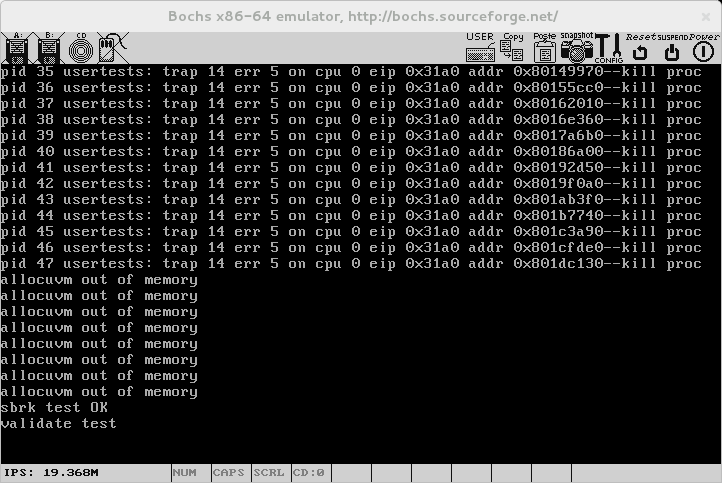
\includegraphics[width=\textwidth]{images/bochs}
	\caption{Bochs running the Muen example system}
	\label{fig:bochs}
\end{figure}

Bochs writes detailed logs during emulation and provides a debugger which allows
to inspect the complete system state at any time. It has proven very helpful
and was invaluable when implementing new low-level processor features.

\section{Example system}\label{sec:example-system}
The Muen project contains an example system that makes use of all the
mechanisms described in the previous sections. Figure \ref{fig:example-system}
shows a schematic overview of the system.

\begin{figure}[h]
	\centering
	\begin{tikzpicture}[node distance=0.33cm]
	\node[redbox, text width=1.5cm, minimum width=2cm, minimum height=2cm] (vts) {VT Native};
	\node[redbox, text width=1.5cm, minimum width=2cm, minimum height=2cm, left=of vts] (cry) {Crypter Native};
	\node[redbox, text width=1.5cm, minimum width=2cm, minimum height=2cm, left=of cry] (smn) {Subject Monitor Native};
	\node[blackbox, text width=1.5cm, minimum width=2cm, minimum height=2cm, left=of smn] (xv6) {xv6 VM};
	\node[bluebox, minimum height=1cm, minimum width=9cm, text width=6cm] at (-3.5,-2.5) (mue) {Muen Separation Kernel};

	\draw[gray] (-8,-2.25) to (1,-2.25);
	\draw[gray] (-5.84,-2.25) to (-5.84,0);
	\draw[gray] (-3.50,-2.25) to (-3.50,0);
	\draw[gray] (-1.14,-2.25) to (-1.14,0);
\end{tikzpicture}

	\caption{Example system}
	\label{fig:example-system}
\end{figure}

The system is composed of the Muen kernel and four subjects, three of which are
trusted and one xv6 subject is untrusted. The trusted subjects run in the native
profile and are implemented in Ada/SPARK, the untrusted xv6 subject runs a teaching
OS written in C inside the VM profile.

The example system is meant to serve as demonstrator for a real-world use-case:
An untrusted operating system is separated by the Muen kernel and accesses
native, trusted services with minimal TCB. The trusted services might even be
formally verified.

The following section explains the different subjects composing the example
system, while section \ref{subsec:keyboard-handling} describes the keyboard
handling in detail to illustrate how the different mechanisms are tied
together.

\subsection{Subjects}

\subsubsection{VT}\label{subsubsec:subject-vt}
The VT subject manages virtual terminal consoles and owns the keyboard. The
system policy therefore assigns the hardware devices shown by listing
\ref{lst:hardware-devs} to the subject. This allows the VT subject to control
the VGA cursor and the contents of the VGA memory. The kernel also programs the
system's I/O APIC so that only the VT subject receives keyboard interrupts (IRQ
1).

\begin{lstlisting}[
	language=xml,
	label=lst:hardware-devs,
	caption=Subject device assignment]
<device name="keyboard" irq="1">
    <io_port start="0060" end="0060"/>
    <io_port start="0064" end="0064"/>
</device>

<device name="vga">
    <memory_layout>
        <memory_region physical_address="b8000" virtual_address="b8000" ...
    </memory_layout>
</device>

<device name="cursor">
    <io_port start="03d4" end="03d5"/>
</device>
\end{lstlisting}

The other subjects of the example system have no direct access to the real VGA
memory but write to a distinct page mapped to their (virtual) VGA memory
address (\emph{0xb8000}). The subject virtual terminal pages are also mapped
into the address space of the VT subject.

If the user hits the special keys F1 to F6, the VT subjects updates the VGA
memory with the contents of the active session slot's virtual terminal page.
All other keyboard scancodes are copied to a driver page shared with the
untrusted xv6 subject and an event is sent to inform it that keyboard data
awaits processing by its virtual keyboard driver.

\subsubsection{Crypter}
The crypter subject uses the libsparkcrypto \cite{libsparkcrypto} library to
provide trusted cryptographic services to clients. On startup, the subject
enters the halted state until it receives an interrupt event indicating a
pending request.

The interrupt event resumes the subject and data contained in the subject's
request page is copied for further processing. Currently, the crypter subject
creates a SHA-256 REF message digest over the received data and then copies the
hash to the service response page. An interrupt event is triggered to signal
service completion.

\subsubsection{xv6}
Xv6\index{xv6} is a Version 6 Unix \cite{wiki:unix6} teaching operating system
developed at MIT \cite{xv6}. While being simple, it implements many key
concepts found in common operating systems, making it an ideal initial target
for the VM profile. Xv6 is written in ANSI C.

Minimal changes in the source code of xv6 were required to run it as VM subject
on the Muen kernel:
\begin{itemize}
	\item Disable MP support
	\item Ignore disallowed I/O operations (handled by the SM subject)
\end{itemize}

Since the xv6 subject has no direct access to the keyboard, a simple virtual
keyboard driver has been implemented.

\subsubsection{Subject Monitor}
The subject monitor (SM\index{SM}) subject is used to monitor the untrusted xv6
subject. It displays information about I/O operations and has complete access to
the architectural state of the xv6 subject. Currently, no emulation is needed to
run xv6. If an unexpected trap occurs, a state dump is output and the virtual
CPU (VCPU\index{VCPU}) is halted.

\subsection{Keyboard handling}\label{subsec:keyboard-handling}
This section describes how the keyboard is handled in the example system using
the mechanisms provided by the Muen kernel.

When pressing a key on the keyboard, the keyboard controller raises an interrupt
request (IRQ\index{IRQ}) with number 1 to signal new data. The system policy
applied by the Muen kernel on startup enforces that this interrupt is routed to
the appropriate processor running the VT subject. This is done using the IRQ
routing specification generated during policy compilation and depends on the
assignment of hardware devices to subjects. In this case, the keyboard is
assigned to subject 1, which is the VT subject described in section
\ref{subsubsec:subject-vt}. Listing \ref{lst:ex-irq-routing} shows the IRQ
routing table of the example system.

\begin{lstlisting}[
	language=Ada,
	label=lst:ex-irq-routing,
	caption=Example system IRQ routing table]
IRQ_Routing : constant IRQ_Routing_Array := IRQ_Routing_Array'(
  1 => IRQ_Route_Type'(
    CPU    => 0,
    IRQ    => 1,
    Vector => 33));
\end{lstlisting}

The routing table contains one entry which routes the keyboard IRQ 1 to the CPU
with APIC ID 0. Furthermore, the IRQ is remapped to the interrupt vector 33 so
that on each key press, CPU0 will be interrupted with an interrupt vector 33.

The Muen kernel running on CPU0 handles the received interrupt in its
\texttt{Handle\_Irq} procedure. It uses the vector routing table contained in
the SPARK-compliant interrupt specification compiled by the \texttt{skpolicy}
tool, see listing \ref{lst:ex-vector-routing}. The table instructs the kernel to
inject interrupt vector 33 into the subject with ID 1 by using the interrupt
injection mechanism described in section \ref{subsec:int-injection}.

\begin{lstlisting}[
	language=Ada,
	label=lst:ex-vector-routing,
	caption=Example system CPU0 vector routing table]
Vector_Routing : constant Vector_Routing_Array := Vector_Routing_Array'(
  33     => 1,
  others => Skp.Invalid_Subject);
\end{lstlisting}

The VT subject receives interrupt vector 33 in its interrupt handling routine
and, because it is allowed to access the respective I/O ports, reads in the
keyboard scancodes. If the received scancode is not related to the special keys
F1 to F6 and the currently visible subject is xv6, the scancode data is copied
into a memory page shared with the xv6 subject. The VT subject then triggers an
event to inform the xv6 subject about new data to process. This is done using
the Muen hypercall mechanism.

The kernel running the VT subject forwards the interrupt event to the respective
subject as defined by the policy. In this case, it is the xv6 subject.

The xv6 subject's interrupt handler code runs unmodified and detects that a
keyboard interrupt has occurred. The appropriate keyboard handling code is
called, which has been slightly modified to read keyboard scancodes from a
shared memory page instead of doing port I/O. The copied scancode data is then
used to drive the terminal console.

